%=-=-=-=-=-=-=-=-=-=-=-=-=-=-=-=-=-=-=-=-=-=-=-=-=-=-=-=-=-=-=-=-=-=-=-=-=-=-=-=-=-=-=-=-=-=
% Preamble - Cal Poly Thesis Based on UC Thesis Format
%=-=-=-=-=-=-=-=-=-=-=-=-=-=-=-=-=-=-=-=-=-=-=-=-=-=-=-=-=-=-=-=-=-=-=-=-=-=-=-=-=-=-=-=-=-=
\documentclass[12pt]{ucthesis}
\usepackage{thesis_preamble}
\usepackage{float}
\title{Flight Testing Small UAVs for Drag Polar Estimation}
\author{Adam Chase}
\degreemonth{September} \degreeyear{2013} \degree{Master of Science}
\defensemonth{September} \defenseyear{2013}
\numberofmembers{4} \chair{Rob McDonald, Ph.D.} \othermemberA{Eric Mehiel, Ph.D.} \othermemberB{Russell Westphal, Ph.D.} \othermemberC{Kurt Colvin, Ph.D.}
\field{Aerospace Engineering} \campus{San Luis Obispo} \copyrightyears{seven}

%=-=-=-=-=-=-=-=-=-=-=-=-=-=-=-=-=-=-=-=-=-=-=-=-=-=-=-=-=-=-=-=-=-=-=-=-=-=-=-=-=-=-=-=-=-=
% Document
%=-=-=-=-=-=-=-=-=-=-=-=-=-=-=-=-=-=-=-=-=-=-=-=-=-=-=-=-=-=-=-=-=-=-=-=-=-=-=-=-=-=-=-=-=-=
\makeatletter
\def\@makechapterhead#1{%
  \vspace*{2\p@}%
  {\parindent \z@ \raggedright \normalfont
    %\ifnum \c@secnumdepth >\m@ne
    %    \huge\bfseries \@chapapp\space \thechapter
    %    \par\nobreak
    %    \vskip 20\p@
    %\fi
    \interlinepenalty\@M
    \huge \bfseries #1\par\nobreak
    \vskip 1\p@
  }}
  \makeatother
  
\begin{document}

\maketitle

\begin{frontmatter}
	
	\copyrightpage
	%\approvalpage
	\committeemembershippage

	\pdfbookmark[0]{Abstract}{abs} % Sets a PDF bookmark for the abstract
\begin{abstract}


\end{abstract}

\begin{acknowledgements}

   Thank you...

\end{acknowledgements}


\addcontentsline{toc}{chapter}{Contents}
\tableofcontents


\listoftables

\listoffigures

\end{frontmatter}

\pagestyle{plain}




\renewcommand{\baselinestretch}{1.66}


% ------------- Main chapters here --------------------


\chapter{Introduction and Motivation}
\label{intro}
An accurate drag prediction is critical for conceptual aircraft design, aircraft mission planning, and predicting performance trends of comparable aircraft. To this end, industry spends an extensive amount of time and money developing wind tunnel models and executing wind tunnel tests. Additionally, it is difficult to impossible to exactly scale down a vehicle, especially when features such as rivets, servo control horns, antennas, and air data probes are included. These differences between the model and the as-built aircraft can cause accuracy of the wind tunnel test to suffer. This inaccuracy inevitably leads to aerodynamic flight tests that attempt to quantify the as-built drag and lift characteristics of the vehicle.
\indent
The flight test of full scale aircraft for drag polar prediction is generally conducted about a trimmed condition. That is, the aircraft is flown to an operating conditions dictated by the test plan, and sets the control surfaces such that there are no accelerations and no moments. Data is then collected for a set amount of time, without changing the operating condition. After the data is collected, the operating point is changed, the aircraft is trimmed at this new flight condition, and data is again collected. This process is repeated at various points in the aircraft's flight envelope until enough data is collected to estimate a drag polar.

\indent
Unfortunately, for many R/C aircraft and small UAVs, this procedure isn't feasible. First, these aircraft typically operate close to ground level, meaning there could potentially be both unsteady and turbulent winds, and a steady wind. R/C aircraft and small UAVs typically have much lower moments of inertias and mass than their full-scale counterparts, which means they will be affected much more by atmospheric disturbances than full-scale vehicles. Second, many of these aircraft have a line-of-sight communication link, and R/C aircraft in particular are flown in small patterns at a flight field. Even in the case of a steady atmosphere, R/C aircraft usually are not well trimmed, because by the time the pilot can see if the vehicle is trimmed, he has to turn around in the pattern. This thesis attempts to fix these problems, by allowing the pilot to fly in a more generic flight path, and not relying on a still atmosphere assumption.

\chapter{Method}

\label{background-information}
Some basic assumptions will apply throughout the modeling of dynamics in thesis. They are as follows:
\begin{enumerate}
\item The vehicle is a fixed mass.
\item Coriolis effects are negligible.
\item Thrust will be assumed to be 0.
\end{enumerate}
Note that a stationary atmosphere is not assumed.

\section{Reference Frames}
For this thesis, the reference frames used will follow those described in \cite{klein2006aircraft}, and will be repeated here for clarity.

\subsection*{North-East-Down (NED) Axes ($x_{ned}$, $y_{ned}$, $z_{ned}$)}
The NED axis system defines a local tangent plane on the Earth's surface, with the origin coinciding with the vehicle's center of gravity. The $\hat{i}$ vector points due north, the $\hat{j}$ vector points due east, and the $\hat{k}$ vector points towards the center of the earth, in accordance with the right-hand rule. This coordinate system is vehicle carried, meaning the origin is fixed, but the axis directions are independent of vehicle orientation.

\subsection*{Body Axes ($x_b$, $y_b$, $z_b$)}
The body axis system has its origin at the vehicle's center of gravity, with the $\hat{i}$ direction pointing out the vehicle's nose, the $\hat{j}$ direction pointing out the right wing, and the $\hat{k}$ direction pointing out the belly of the aircraft, in accordance with the right-hand rule. This coordinate frame is fixed to the body, meaning the aircraft's spatial orientation does not change the direction of the axes.

\subsection*{Stability Axes ($x_s$, $y_s$, $z_s$)}
The stability axes are defined with its origin coinciding with the center of gravity of the vehicle. This axis system has essentially the same directions as the body axes, except rotated about the body axis $\hat{j}$ through an initial angle-of-attack, $\alpha_{0}$. This inital angle-of-attack is defined at the beginning of a test maneuver and is then set for the remainder of the test, making it a body-fixed coordinate system. This system assumes no initial sideslip angle \cite{roskam2001airplane}.

\subsection*{Wind Axes ($x_w$, $y_w$, $z_w$)}
The wind axes are, again, a vehicle-carried coordinate system, meaning the origin of the wind axis also coincides with the center of gravity of the vehicle. However, the wind axes are not a body-fixed coordinate frame. The $\hat{i}$ direction points into the oncoming air, as seen from the vehicle. The $\hat{k}$ direction lies in the x-z plane of the body reference frame. The $\hat{j}$ direction is then defined to be out the right side of the vehicle, in order to follow the right hand rule. 

\section{Equations of Motion}
\label{sys-desc}
Newton's 2nd Law of Motion states
\begin{align}
\vec{F} &= \frac{d}{dt}(m\vec{V})
\end{align}
where $\vec{F}$ is the sum of all applied forces, $\vec{m}$ is the mass of the vehicle, and $\vec{V}$ is the vehicle's velocity. Using the fixed mass assumption, this reduces to 
\begin{align}
\vec{F} &= m\frac{d\vec{v}}{dt}\\
&= m\vec{a}
\end{align}

The applied forces on the vehicle are 
\begin{align}
\vec{F} &= \vec{F}_{A}+\vec{F}_{G}+\vec{F}_{T}
\end{align}

where $\vec{F_{A}}$ accounts for all aerodynamic forces acting on the vehicle, $\vec{F_{G}}$ is the force due to gravity, and $\vec{F_{T}}$ accounts for forces from the propulsion system. Each of these forces will be discussed next.

\subsection*{Aerodynamic Forces}
Aerodynamic forces are described in the stability reference frame. In general, they are defined as

\begin{align}
\vec{F}_{A_S} &= D \hat{i}_s+Y \hat{j}_s+L \hat{k}_s
\end{align}

where $D$ is drag force, $Y$ is side force, and $L$ is lift force. 

\subsection*{Gravitational Forces}
The gravitational force on the vehicle acts in the $+z_{ned}$ direction and is equal in magnitude to the vehicle's weight $W$, leading to
\begin{align}
\vec{F}_{G_{ned}} &= 0\hat{i}_{ned}+0\hat{j}_{ned}+W\hat{k}_{ned}
\end{align}

\subsection*{Propulsive Forces}
In general, propulsive forces are modeled as
\begin{align}
\vec{F}_{T_b} &= T_x \hat{i}_b+T_y \hat{j}_b +T_z \hat{k}_b
\end{align}
where $T_x$, $T_y$, and $T_z$ are components of thrust in their respective body axis directions. However, as previously mentioned, propulsive forces are assumed to be $\vec{0}$ for this thesis.

\subsection{Combined Forces in Body Axes}
The forces are combined and transformed into the body axes reference frame so that they align with the output of body mounted accelerometers. The combined equations of motion are then

\begin{align}
\vec{F}_{AERO_W} = DCM_{bw}^{-1}(m\vec{a} - DCM_{ib}\vec{F}_{GRAVITY_i})
\end{align}


\section{Kalman Filter Usage}
\label{kalman-filter}
This thesis utilizes multiple Kalman Filters to estimate both regression coefficients and improved states. The Kalman filter operates recursively on a time-series and provides an optimal estimate of the system state.

\subsection{Linear Kalman Filter}
A linear Kalman filter can be applied where the system in question can be described in the form \cite{welch1995introduction}

\begin{align}
x_k &= Ax_{k-1} + Bu_{k-1}+w_{k-1}
\end{align}
where $A$ is the state transition matrix, $x_{k-1}$ is the previous state, $B$ is the input matrix, $u_{k-1}$ is the input vector, and $w_{k-1}$ is random process noise.

The measured state is then 
\begin{align}
z_k &= Hx_k+v_k
\end{align} 

where $H$ is the output matrix and $v_k$ is measurement noise.

\indent
The Kalman filter operates in a predictor-corrector manner, where the predictor step is often called the \textit{a priori} estimate, and the corrector step is often called the \textit{a posteriori} estimate. The \textit{a priori} state estimate is calculated using prior states and inputs, while assuming no process noise

\begin{align}
\hat{x}^-_k &= A\hat{x}_{k-1}+Bu_{k-1}
\end{align}



The \textit{a priori} estimate of the covariance matrix is projected in a similar manner

\begin{align}
P^-_k &= AP_{k-1}A^T+Q
\end{align}

where Q the process noise covariance matrix.

The Kalman gain is calculated by combining the predicted, \textit{a priori} covariance matrix with the measurement noise covariance matrix $Q$

\begin{align}
K_k &=P^-_kH^T(HP^-_kH^T + R)^{-1}
\end{align}

This optimal Kalman gain is then used to estimate the \textit{a posteriori} estimate of the state and covariance matrix

\begin{align}
\label{kalmanStateUpdate}
\hat{x}_k &=\hat{x}^-_k+K_k(z_k-y_k)
\end{align}

\begin{align}
P_k &= (I-K_kH)P^-_k
\end{align}

where $y_k$ is the predicted value of $z_k$ found using the output matrix $H$ and the \textit{a priori} state estimate
\begin{align}
y_k &= H\hat{x}^-_k
\end{align}
Note that Equation \ref{kalmanStateUpdate} is essentially a weighted average of a measured state and an expected state. The weighting is the Kalman gain, which is related to the ratio of confidence in the measured state and the expected state. For a 1-D case with equal confidence between the measured state and the expected state, the Kalman gain $K_k = 0.5$, and the Kalman filter becomes a simple and straight-forward average.


\subsection{Extended Kalman Filter}
\label{EKFTheory}
The Extended Kalman filter is used for a non-linear system and is essentially a linearization of a nonlinear plant. A non-linear system can be described as \cite{welch1995introduction}

\begin{align}
x_k &= f(x_{k-1},u_{k-1},w_{k-1})\\
z_k &= h(x_k,v_k)
\end{align}

The process noise $w_{k-1}$ and measurement noise $v_k$ are not known (or the Kalman filter would not be necessary), so the states are approximated assuming both noise sources are 0

\begin{align}
\tilde{x}_k &= f(\hat{x}_{k-1},u_{k-1},0)\\
\tilde{z}_k &= h(\tilde{x}_k,0)
\end{align}

The actual states are related to the approximate states by

\begin{align}
x_k &\approx\tilde{x}_k+A(x_k-\hat{x}_{k-1})+Ww_{k-1}\\
z_k &\approx\tilde{z}_k+H(x_k-\tilde{x}_{k-1})+Vv_k
\end{align}

where  the matrices $A$, $W$, $H$, and $V$ represent the different Jacobians matrices:
\begin{align}
A &= \frac{\partial f_i}{\partial x_j}(\hat{x}_{k-1},u_{k-1},0)\\
W &= \frac{\partial f_i}{\partial w_j}(\hat{x}_{k-1},u_{k-1},0)\\
H &= \frac{\partial h_i}{\partial x_j}(\hat{x}_{k},0)\\
V &= \frac{\partial h_i}{\partial v_j}(\hat{x}_{k},0)
\end{align}

The Extended Kalman Filter uses these linearized equations to perform the same process as the linear Kalman Filter. Again, the first step is to calculate the \textit{a priori} estimate of the state and the covariance matrix
\begin{align}
\hat{x}^-_k &=f(\hat{x}_{k-1},u_{k-1},0)\\
P^-_k  &= A_kP_{k-1}A^T_{k-1}+W_kQ_{k-1}W^T_k
\end{align}

Next, the Kalman gain is calculated
\begin{align}
K_k &=P^-_kH^T_k(H_kP^-_kH^T_k+V_kR_kV^T_k)^{-1}
\end{align}

The Kalman gain is then used to calculate the \textit{a posteriori} estimate of the state and covariance matrix

\begin{align}
\hat{x}_k &=\hat{x}^-_{k}+K_k(z_k-y_k)\\
\label{kalmanVariance}
P_k &=(I-K_kH_k)P^-_k
\end{align}

where $y_k$ is, as in the linear case, the predicted value of $z_k$, but calculated using the nonlinear output function and the \textit{a priori} state estimate

\begin{align}
y_k &= h(\hat{x}^-_k,0)
\end{align}

Unlike the linear Kalman filter, the Extended Kalman filter is not proven to be optimal. However, it has been utilized for a wide range of applications with excellent results.

\chapter{Regression Model}
The purpose of this thesis is to reduce flight test data into a meta-model that can be used to predict performance information about the aircraft. Therefore, the regression model used to estimate the meta-model is critical. 

\section{Regression Model - Least Squares Fit}
The standard model for polynomial regression is

\begin{align}
\label{polyRegress}
\hat{y} &= \beta_0 + \beta_1x + \beta_2x^2+...
\end{align}

For a parabolic estimation of the drag polar of an aircraft, equation \ref{polyRegress} becomes
\begin{align}
C_D = C_{D_0} + K_1 C_L+K_2 C^2_L
\end{align}

These coefficients can be estimated using an Ordinary Least Squares fit. The Ordinary Least Squares problem statement is as follows
\begin{align}
\bar{A}\vec{x} &= \vec{b}
\end{align}
If $\bar{A}$ is an $m$x$n$ matrix of measured state data, $\vec{x}$ is an $n$x$1$ vector of correlation coefficients, and $\vec{b}$ is an $m$x$1$ vector of measured function data, the solution to the Ordinary Least Squares problem is 

\begin{align}
\bar{A}\vec{x}&=\vec{b}\\
\bar{A}^T\bar{A}\vec{x} &= \bar{A}^T\vec{b}\\
(\bar{A}^T\bar{A})^{-1}(\bar{A}^T \bar{A})\vec{x} &= (\bar{A}^T\bar{A})^{-1}\bar{A}^T\vec{b}\\
\bar{I}\vec{x} &=(\bar{A}^T\bar{A})^{-1}\bar{A}^T\vec{b}
\end{align}

When applied to estimating a parabolic drag polar, the $\bar{A}$ matrix becomes
\begin{align}
\bar{A}_{i,:} &= 
\begin{bmatrix}
1 & C_{L_i} & C^2_{L_i}
\end{bmatrix}
\end{align}
the $\vec{b}$ vector becomes

\begin{align}
\vec{b}_i &=
\begin{bmatrix}
C_{D_i}
\end{bmatrix}
\end{align}

and the $\vec{x}$ vector, which is the vector of interest, becomes
\begin{align}
\vec{x} &=
\begin{bmatrix}
C_{D_0} & K_1 & K_2
\end{bmatrix}^T
\end{align}

which are the coefficients of interest for the regression model.
\section{Regression Model - Kalman Filter}
The coefficients in question can also be estimated using an Extended Kalman filter. The system can again be described as 

\begin{align}
C_D &= C_{D_0}+K_1C_L+K_2C^2_L
\end{align}

For the Kalman filter regression, the state to be estimated are the coefficients $C_{D_0}$, $K_1$, and $K_2$. Since the regression coefficients should not change, the state transition matrix is an identity matrix, leading to

\begin{align}
\hat{x}_k &= \begin{bmatrix}
C_{D_0} & K_1 & K_2
\end{bmatrix}\\
A &= \begin{bmatrix}
1&0&0\\0&1&0\\0&0&1
\end{bmatrix}
\end{align}


The measured data $z_k$ is a vector containing the lift and drag coefficients at the $k$-th instant in time

\begin{align}
z_k &= \begin{bmatrix}
C_D\\C_L
\end{bmatrix} &= h(x_{k},0)
\end{align}


The vector $y_k$ contains the estimates of $C_D$ and $C_L$ found using the \textit{a priori} state vector $\hat{x}^-_k$ and is equal to

\begin{align}
y_k &= \begin{bmatrix} C^-_{D_{0_k}}+K^-_{1_k}C_L+K^-_{2_k}C^2_L \\ C_L \end{bmatrix} &=h(x^-_k,z_k,0)
\end{align}


To implement into the Extended Kalman filter, the Jacobian of $h(x^-_k,z_k,0)$ with respect to $x_k$ needs to be calculated. Once done, the $H$ matrix in the EKF becomes

\begin{align}
H_k = \begin{bmatrix}
1 & C_L & C^2_L\\0&0&0
\end{bmatrix}
\end{align}


With the $H$ matrix calculated, the EKF algorithim can be implemented as described in Section \ref{EKFTheory}. The measurement noise covariance at each instant was calculated by doing error propagation as described in Section \ref{pointError} and the process noise covariance was set to zero because the coefficients should be exactly constant.

\chapter{Error Analysis}
When discussing error, there are two main types: model regression error and the error of a single data point. The error of a single data point comes from random noise in sensors, and can be decreased by improving the accuracy of the sensor or filtering the results. The model regression error comes from the fact that every aspect of the dynamics of the system are not precisely modeled. This type of error can be reduced by improving the accuracy of the dynamics being modeled or by increasing the amount of data being taken.
\section{Random Error}
\label{pointErrorSection}
Without estimates of the error in data, the data itself is fairly meaningless. The equations of motion can be used to propagate uncertainty in a signal through, and allows the uncertainty in the coefficients to be estimated based on sensor noise. The noise can be either systematic or random. Systematic error can be caused by many things, including poorly modeled physics and a steady-state offset of a sensor. Random error is due to the inherent inaccuracy of the sensors, and is generally assumed to be normally distributed.

The error of a single point is assumed to be random error and normally distributed. The first step in error propagation is to define the $y_i$ to be the $i$-th entry of the true function vector, $\hat{y_i}$ to be the $i$-th entry of the measured function vector, and to then do a Taylor series expansion about the operating point.
\begin{align}
\hat{y_i} &= y_i + \frac{\partial{y_i}}{\partial{x_j}}dx_j+HOT
\end{align}
where $x_j$ is the $j$-th element of the state vector and $HOT$ represents the truncated  \textbf{H}igher \textbf{O}rder \textbf{T}erms of the Taylor series. Note that the term $\frac{\partial{y_i}}{\partial{x_j}}$ is the Jacobian ($\bar{J_{ij}}$) matrix of the state transition function. The error can then be defined as (dropping $HOT$)
\begin{align}
\label{contErrorEqn}
dy_i &= \hat{y_i}-y_i =  \bar{J_{ij}}dx_j
\end{align}
If the error is then interpreted as a discrete difference instead of a continuous difference, equation \ref{contErrorEqn} becomes
\begin{align}
\label{errorEqn}
\Delta y_i &= \bar{J_{ij}}\Delta x_j
\end{align}

If the $\Delta$ values are further assumed to represent standard deviations of normally distributed error, equation \ref{errorEqn} becomes
\begin{align}
\sigma_{y_i} &= \bar{J_{ij}} \sigma_{x_j}
\end{align}
For the purposes of this thesis, $\sigma_{y_i}$ is a vector of the standard deviations of the aerodynamic force coefficients,
\begin{align}
\sigma_{y_i} &= \begin{bmatrix} \sigma_{C_{D_i}} & \sigma_{C_{Y_i}} & \sigma_{C_{L_i}} \end{bmatrix}^T
\end{align}

and $\sigma_{x_j}$ is a vector of the standard deviations of the state values,
\begin{align}
\sigma_{x_j} &= \begin{bmatrix} \sigma_{\bar{a}_j} & \sigma_{\alpha_j} & \sigma_{\beta_j} & \sigma_{\bar{\omega}_j} & \sigma_{\phi_j} & \sigma_{\theta_j} & \sigma_{\psi_j}\end{bmatrix}^T
\end{align}
For initial error estimation, the noise levels reported by instrument manufacturers was assumed to be one standard deviation. The Jacobian matrix was calculated at each observed data point and combined with the sensors standard deviation to produce estimates of the standard deviations of the aerodynamic coefficients.

One of the key findings of this section is that the error of the coefficient depends on the coefficient itself. This means that the error varies from data point to point, which is called \textit{heteroskedasticity}. To account for this, an error estimate function was created in Matlab, which used the error propogation outlined in this section. This function was used whenever an estimate of point error was required, such as the variance matrix $P_k$ used in the Kalman filters utilized for state estimation. A plot of simulated flight data is shown in Figure \ref{errorBndFigure}, where the error bounds shown were calculated using the error estimate function. Note that this figure also shows the heteroskedastic nature of the error.

\begin{figure}[h!]
  \caption{Heteroskedastic Error from Simulated Flight} \label{errorBndFigure}
  \centering
    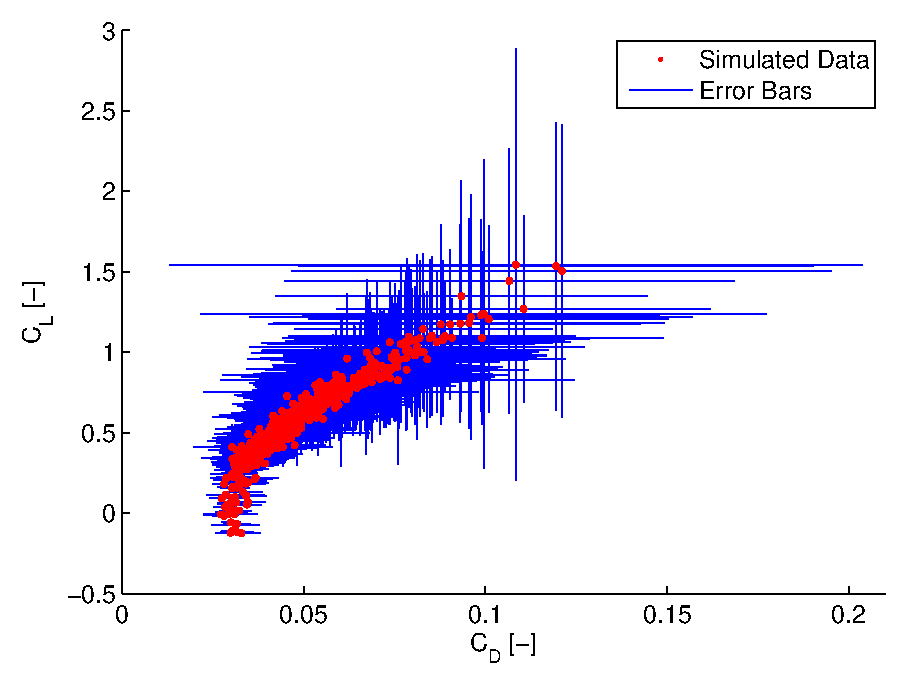
\includegraphics[width=0.5\textwidth]{figures/heteroskedasticity.eps}
\end{figure}

Additionally, while heteroskedasticity does not color the estimate of $\hat{\beta}_i$, it does color the confidence intervals. The method of dealing with this problem is discussed in Section \ref{leastSquaresError}.


\section{Least Squares Model Error}
\label{leastSquaresError}
The error of a single data point is not the main driving factor in the accuracy of a regression model. The important factors in the model are how accurate the coefficients are known, which is a function of the accuracy of each point, as well as the number of points sampled. The main parameter that describes the accuracy of the regression coefficients are the confidence intervals. A confidence interval is a range of values such that, if the experiment were repeated, the parameter calculated would be within the range some percentage of the time. So, a parameter can be represented as an estimated value, with a confidence bound

\begin{align}
\label{confidenceInterval}
\beta &= \beta_{EST} \pm t\frac{\sigma}{\sqrt{n}}
\end{align}

where $\beta$ is the parameter in question, $\beta_{EST}$ is the estimated value of the parameter, $t$ is the $t$ value based on the number of samples and the desired confidence interval, $\sigma$ is the standard deviation of the sample, and $n$ is the number of data points collected. Since  the number of data points collected will be large ($>100$) in this thesis, the $t$ value will be taken as 1.96 for a 95\% confidence interval.

\indent

As previously mentioned in Section \ref{pointErrorSection}, one of the assumptions made in a Least Squares regression is homoskedasticity. However, the error using standard uncertainty propogation is heteroskedastic. This becomes a problem in estimating confidence intervals, because the standard error can be driven by outliers. If each data point had the same error, these outliers could be valid. However, if the data is heteroskedastic, the outlier may have a larger error bound, meaning the data point isn't as unlikely as it first appears. This fact can drive the standard error estimate to be larger than is appropriate, which leads to a larger confidence interval and possibly a false acceptance of the confidence interval's hypothesis test. To account for this, Matlab's ``robustfit" function was used to estimate both the coefficients and robust standard error estimates. The ``robustfit" function calculates robust standard error estimates by doing a weighted average where the weighting is based on a radial basis function. This means that the farther away a data point is from the estimated regression model, the less impact it has on the standard error of the model. Some weighting functions for the weight $w$ that are available in Matlab's ``robustfit" are shown below.

\begin{align}
\text{``Cauchy"} &: w = \frac{1}{1+r^2}\\
\text{``Bisquare"} &: w = \text{logical}(|r|<1)*(1-r^2)^2\\
\text{``Fair"} &: w =\frac{1}{1+|r|}\\
\text{``Welsch"} &: w = e^{-r^2}
\end{align}

The default weighting function used by ``robustfit" is bisquare, so it was used for this thesis.

\section{Kalman Filter Error}
Kalman filters are often used to propagate states. The filter does this by combining the system dynamics with a measured state. The variance is propagated using Equation \ref{kalmanVariance}. When estimating coefficients using the Kalman filter, the $\bar{A}$ state transition matrix is an identity matrix, which is due to the fact that the coefficients stay constant. When propagated through the filter, this means the variance estimate $P_k$ is essentially a variance-weighted-average of the coefficient estimates. The resulting matrix $P_k$ contains the variance of the coefficient estimates. Equation \ref{confidenceInterval} calculates the confidence interval of regression coefficients and needs the standard deviation of the mean, also called the standard error. The matrix $P_k$ can be used  to calculate the confidence intervals by noting

\begin{align}
P_k &= \begin{bmatrix}
\sigma_{1}^2 &  0  & \ldots & 0\\
0  &  \sigma_{2}^2 & \ldots & 0\\
\vdots & \vdots & \ddots & \vdots\\
0  &   0       &\ldots & \sigma_i^2
\end{bmatrix}
\end{align}

The confidence interval for coefficient $\beta_i$ can be calculated using $\sigma_i$ in Equation \ref{confidenceInterval}.

\chapter{Simulation}
\label{simulation}
A 6-DOF flight simulator was used to validated the drag prediction method before hardware was purchased. The main utility of the simulator was to provide simulated flight test data with signals that contained no noise. The actual sensors during a flight test will be noisy signals, and Guassian white noise can be added to the clean signals to check the method's sensitivity to sensor noise.

\section{Simulation Environment}
The flight simulator used was a model of the de Haviland Beaver that comes as a demo in the Aerospace Toolbox of Simulink. The Simulink model was modified to output required signals to the workspace, which essentially created a sensor with zero noise. The mass, moments of inertia, and reference lengths were then scaled to those of a Zagi R/C aircraft found in \cite{stevens2003aircraft}. The original Simulink model was already connected to a Flight Gear visualization engine, but the model was altered such that the indicators would function properly.

\section{Simulation Inputs}
The engine forces and moments were set to zero in the simulator, to match the assumption of a folding propeller.
The force calculations built into the Beaver Simulink model were replaced with a parabolic drag polar of the form
\begin{align}
C_D &= C_{D_0} + K*(C_L(\alpha)-C_{L_{min}})
\end{align}

The lift coefficient $C_L(\alpha)$ was nonlinear aerodynamic data from a NACA 0012 taken from \cite{osborne2007transitions}. While this approximation to a nonlinear drag polar does not capture the drag rise due to stall, it does represent the limited lifting capability of a real wing, making it more realistic than assuming the wing does not stall.
\section{Simulation Results}
The most first result of the simulation testing was a verification of the correct equations of motion. The simulation was initialized with various initial states to ensure there was no dependence on initial conditions. The vehicle was then flown by an R/C aircraft pilot using a joystick attached the to simulation. It was noted early in the simulation testing that flying a sweep of speeds was beneficial, as a wider range of the drag polar was flown. This result was included in much of the flight test planning.
One of the main goals of the simulation was to verify the data analysis routines developed in Matlab did in fact match inputs to outputs. To do this, the simulation was flown and, when finished, no noise was added to the data. The results are shown in Figure \ref{dragPolarNoNoise}.

\begin{figure}[h!]
  \caption{Equations of Motion Verification (No Noise)} \label{dragPolarNoNoise}
  \centering
    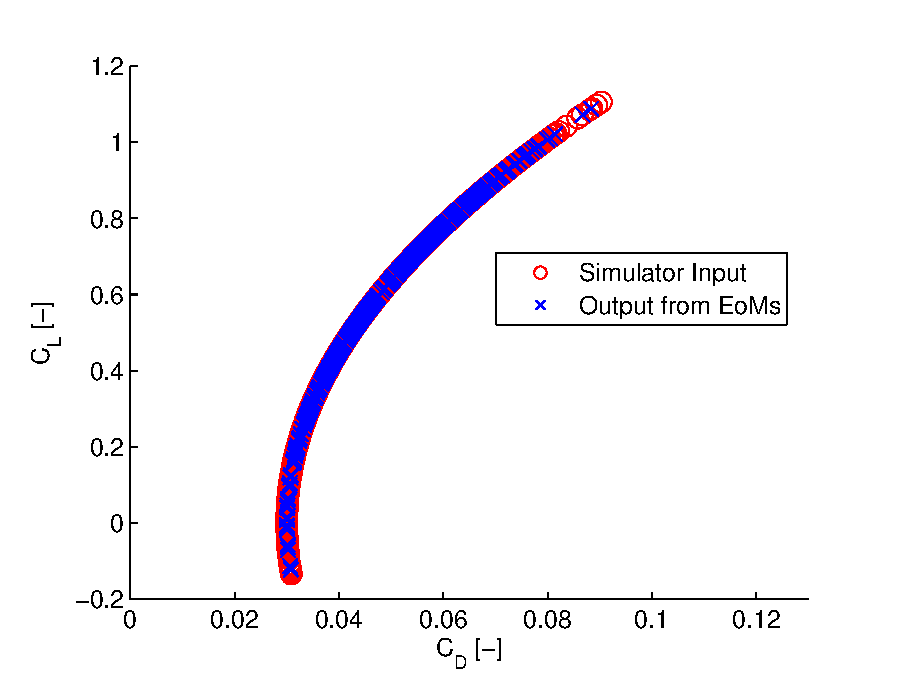
\includegraphics[width=0.5\textwidth]{figures/dragPolarNoNoise.eps}
\end{figure}

Figure \ref{dragPolarNoNoise} shows that the equations of motion used in the data analysis functions properly calculate the coefficients being passed into the system. With this result, noise was added to the system to see how sensitive coefficient estimation was to noise in each sensor. This process was a balancing act between available sensor accuracy and accuracy of the final solution. The final result guided sensor selection to those discussed in Section \ref{hardware}. To check if the final sensors chosen were acceptable, Gaussian noise was added to each state, with a mean of $0$ and a standard deviation equal to the root-mean-squared error listed in the manufacturer's data sheet for each sensor.
\begin{figure}[H]
  \caption{Drag Polar Prediction of Simulated Test Flight} \label{dragPolarNoise}
  \centering
    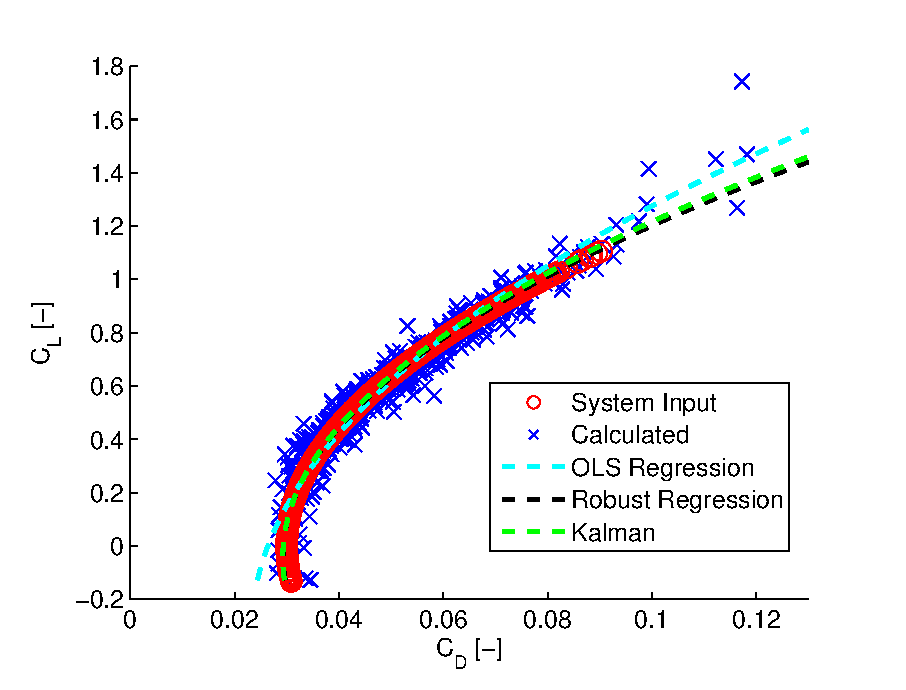
\includegraphics[width=0.5\textwidth]{figures/simDragPolarNoise.eps}
\end{figure}

For the particular simulated test flight shown in Figure \ref{dragPolarNoise}, the estimated drag polar coefficients had error coefficients outlined in Table \ref{simCoeffErrorTable}.

\begin{table}[ht]
\caption{Nonlinear Model Results} % title of Table
\centering % used for centering table
\begin{tabular}{c c c c} % centered columns (4 columns)
\hline\hline %inserts double horizontal lines
 & $C_{D_0}$ & $K_1$ & $K_2$ \\ [0.5ex] % inserts table 
%heading
\hline % inserts single horizontal line
System Inputs & 0.0493 & 0 & 0.03 \\ % inserting body of the table
OLS Estimate & 0.0516 & -0.0056 & 0.0317 \\
Robust LS Estimate & 0.0500 & -0.0035 & 0.0313 \\ [1ex] % [1ex] adds vertical space
\hline %inserts single line
\end{tabular}
\label{table:nonlin} % is used to refer this table in the text
\end{table}

The results of this simulated flight test showed that the measurement system outlined in Section \ref{hardware} predicted the simulated drag polar with a reasonable error.
\chapter{Hardware}
\label{hardware}
Hardware selection was approached from a ``minimum sensor" perspective. One of the main goals of this thesis was to reduce the number of sensors as much as possible to increase the variety of aircraft the hardware can fly on. To accomplish this, sensors were separated based on which state they could estimate.
\section{Accelerations}
The accelerometer chosen for this thesis was the ADXL-362 from Analog Devices. It has a noise error of $175\mu\text{g}/\sqrt{\text{Hz}}$ and has a 3.3V digital SPI interface\cite{adxl362DataSheet}.
\section{Vehicle Mass}
All test vehicles will be weighed using a U-Line H-1650 counting scale. The scale has an accuracy of 0.001 lbs and a maximum capacity of 30 lbs. The minimum capacity of the scale is 10 grams \cite{U-Line}.
\section{Euler Angles}
The Euler angles of the aircraft can be estimated using either an 3-d electronic compass or a 3-d mangetometer. A magnetometer reads the direction and magnitude of a magnetic field, while a compass combines a magnetometer with accelerometer readings to produce a more accurate estimate of the true angles. A Honeywell HMR-3500 3-d electronic compass was used for this thesis. 

\begin{figure}[H]
  \caption{TruePoint™ Compass Module 
  HMR3500 } \label{hmr3500Picture}
  \centering
    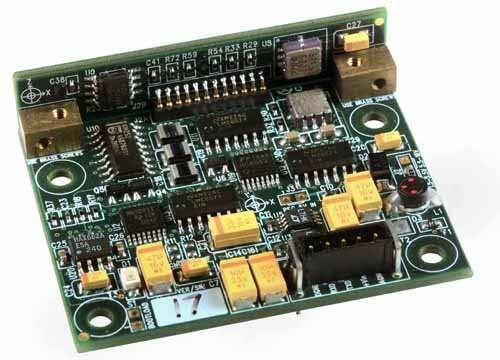
\includegraphics[width=0.5\textwidth]{figures/hmr3500.jpg}
\end{figure}

This compass provides a standard deviation of repeatability in roll of $0.2^\circ$ and a standard deviation of repeatabiltiy in pitch of $0.1^\circ$. Additionally, the heading accuracy is typically a standard deviation of $0.5^\circ$ \cite{honeywellHMR3500}. 

\subsection*{Euler Angle Kalman Filter}
For increased accuracy, a discrete linear Kalman filter is applied. This necessitated adding a three-axis gyroscope to the system. The gyroscope chosen was the Invensense ITG-3200. This gyroscope has a total error of $0.38^\circ/$s-rms, and uses a digital I$^2$C interface that can have its logic level voltage defined on an input pin. The gyroscope has a selectable full-scale span that goes up to $\pm2000^\circ/$s. The gyroscope was purchased in breakout board form from Sparkfun Electronics \cite{itg3200DataSheet}.

\begin{figure}[H]
  \caption{Sparkfun's ITG-3200 Gyroscope Breakout Board} \label{itg3200Picture}
  \centering
    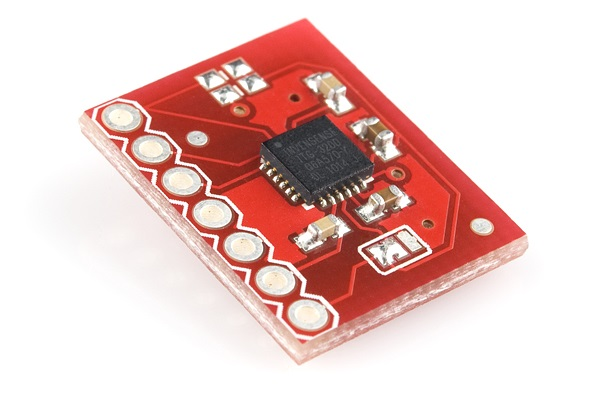
\includegraphics[width=0.5\textwidth]{figures/itg3200.jpg}
\end{figure}

With the angular rates available from the gyroscope, the system equations for the Kalman filter are
\begin{align}
\begin{bmatrix}
\phi_{k}\\
\theta_{k}\\
\psi_{k}
\end{bmatrix} & = \begin{bmatrix}
1 & 0 & 0\\0 & 1 & 0\\0 & 0 & 1
\end{bmatrix}\begin{bmatrix}
\phi_{k-1}\\
\theta_{k-1}\\
\psi_{k-1}
\end{bmatrix}
+ \begin{bmatrix}
\Delta T & 0 & 0 \\ 0 & \Delta T & 0\\0 & 0 & \Delta T
\end{bmatrix}\begin{bmatrix} 
p_k \\ q_k \\ r_k 
\end{bmatrix}+\hat{w}_{k-1}\\
z_k & = \begin{bmatrix}
1 & 0 &0\\0&1&0\\0&0&1
\end{bmatrix}\begin{bmatrix}
\phi_{k}\\
\theta_{k}\\
\psi_{k}
\end{bmatrix}+\hat{v}_{k-1}
\end{align}

The measurement covariance noise matrix was calculated using the standard deviation of the calibration data for the magnetometer, and the process noise covariance matrix was calculated using the standard deviation of the calibration data for the rate gyroscope.
\section{Wind Angles}
The accuracy at which the aerodynamic wind angles are calculated is critical to the overall prediction accuracy. In keeping with the goal of minimizing the number of required sensors, an attempt was made to estimate aerodynamic angles without directly measuring them. There has been a plethora of work conducted on this subject. One of the first available papers on the subject was from the Air Force Institute of Technology \cite{joseph1988}. In that paper, two methods were developed: one for in flight estimation, and the other for post-flight estimation. Both methods relied on either estimated or known stability derivatives. Since the purpose of this thesis is to estimate part of the dynamics, this estimating scheme will not work. Other techniques assume linearization about an operating condition \cite{morelli2012real}. For R/C aircraft this assumption generally cannot be made due to visual flight rules. Other work \cite{Lie2013} combined a dynamics model and a no-vertical-wind assumption. The overarching theme of this previous estimation work was that too many assumptions needed to be made to get results that were not accurate enough ($\approx1^\circ-2^\circ$) for drag polar estimation. For this reason, it was necessary to directly measure airflow angles.

\indent
A five-hole probe was chosen to measure aerodynamic angles as they do not contain moving parts and can provide very accurate, repeatable data. The five-hole probe selected was the Aeroprobe Air Data probe. It has a length of 6 inches and a diameter of 1/8 inch and has an integrated thermocouple for temperature measurement. Each line of the air data probe is connected to a Honeywell Integrated Pressure Transducer (IPT), model number IPT0001D33R. 

\begin{figure}[H]
  \caption{Honeywell Integrated Pressure Sensor} \label{honeywellIPTPicture}
  \centering
    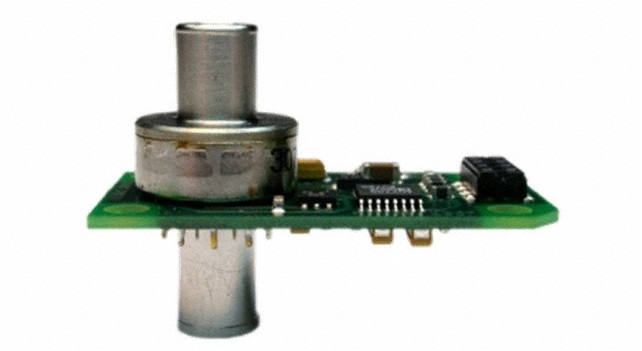
\includegraphics[width=0.5\textwidth]{figures/honeywellIPT.jpg}
\end{figure}

These are 1 PSI differential pressure sensors with a total error band of 0.2\% of full scale. They have a digital SPI interface that operates on a 3.3V logic level and output both a 24-bit pressure and a 16-bit temperature readings \cite{HoneywellIPTDataSheet}.
\subsection{Calibration}
The five-hole air-data probe is calibrated using a Cal-Jet.
\subsection{Wind Angle Kalman Filter}

To improve the accuracy of the wind angle estimation, a discrete, an Extended Kalman filter was used. The state transition functions are nonlinear and are
\begin{align}
\dot{\alpha} & = \frac{1}{V\cos\beta}(-a_x\sin\alpha+a_z\cos\alpha)+q-(p\cos\alpha+r\sin\alpha)\tan\beta\\
\dot{\beta} &=\frac{1}{V}(-a_x\cos\alpha\sin\beta+a_y\cos\beta-a_z\sin\alpha\sin\beta)+p\sin\alpha-r\cos\alpha
\end{align}

The equations for the Kalman filter for the wind angles are
\begin{align}
\begin{bmatrix}
\alpha_k\\\beta_k
\end{bmatrix} &= \begin{bmatrix}
1& 0\\0&1
\end{bmatrix}\begin{bmatrix}
\alpha_{k-1}\\\beta_{k-1}
\end{bmatrix}+\begin{bmatrix}
\Delta T& 0\\0&\Delta T
\end{bmatrix}\begin{bmatrix}
\dot{\alpha_{k}}\\\dot{\beta_{k}}
\end{bmatrix}+\hat{w}_{k-1}\\
z_k & = \begin{bmatrix}
1 & 0\\0&1
\end{bmatrix}\begin{bmatrix}
\alpha_{k}\\
\beta_{k}
\end{bmatrix}+\hat{v}_{k-1}
\end{align}

The process covariance matrix was calculated using the error propogation discussed in Section \ref{pointErrorSection} and the standard deviation data from calibration of each of the sensors. The measurement noise covariance matrix was calculated based on the standard deviation data for the 5-hole probe calibration.

\section{Flight Computer}
The flight computer chosen was an Arduino Due. This board has a 32-bit ARM processor, 54 digital I/O pins, 12 analog input pins, and 2 analog output pins. 

\begin{figure}[H]
  \caption{Arduino Due Flight Computer} \label{arduinoPicture}
  \centering
    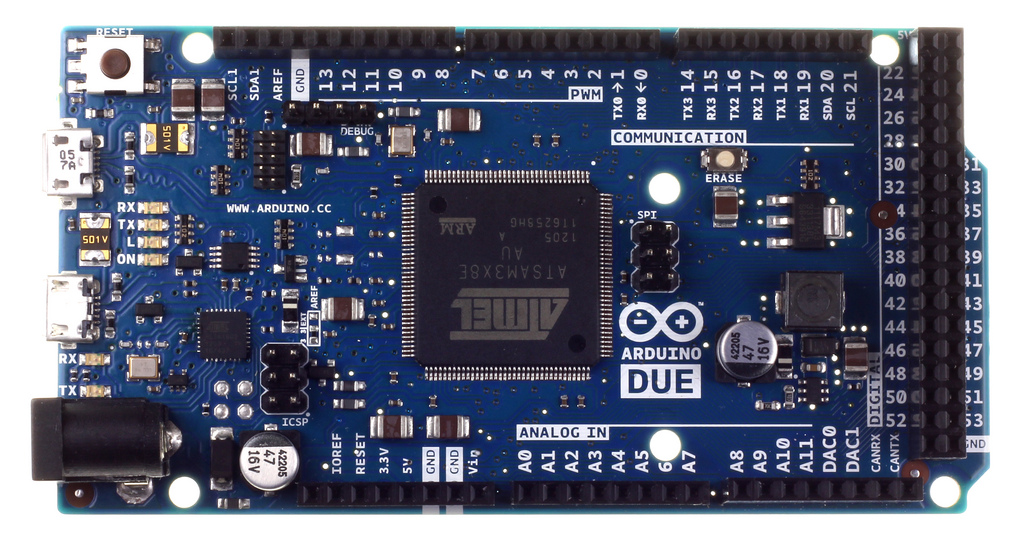
\includegraphics[width=0.5\textwidth]{figures/arduinoDue.jpg}
\end{figure}

One of the main differences between this board and other Arduinos is that the Due operates on a 3.3V logic level instead of the normal 5V. This means sensors such as the HMR-3500 compass need logic level converters. To this end, logic level converters were purchased from Sparkfun. They are 2 channel, bi-directional converters and come in breakout board form.

\begin{figure}[H]
  \caption{Sparkfun Logic-Level Converter} \label{logicLevelConverter}
  \centering
    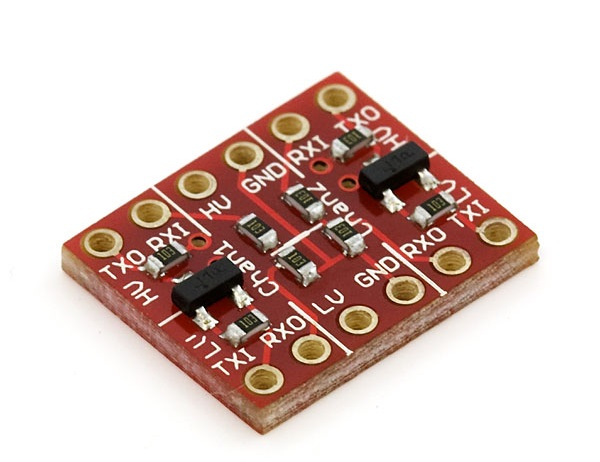
\includegraphics[width=0.5\textwidth]{figures/logicLevelConverter.jpg}
\end{figure}

While the Arduino Due operates a 3.3V digital I/O system, it does provide a 5V source. This source powers the higher voltage side of the logic-level converter

\section{Additional Sensors}
A uBlox LEA-6T GPS receiver was included in the data acquisition system to aid in mission visualization. This model was selected for its ability to output raw timing data, which can be used to get an extremely accurate inertial velocity estimate\cite{ubloxDemo}. The receiver itself was integrated onto a board sold by CGS Shop and has UART,USB, and I$^2$C interface options.

\begin{figure}[H]
  \caption{CGS Shop Board for uBlox LEA-6T} \label{gpsPicture}
  \centering
    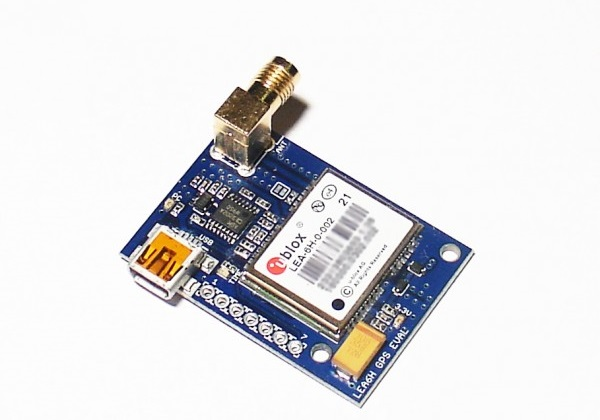
\includegraphics[width=0.5\textwidth]{figures/gpsBoard.jpg}
\end{figure}

A barometric altitude sensor was also included the data acquisiton system. The model chosen was another Honeywell IPT, model number IPT0020A33. This sensor has reads absolute pressures to 20 PSI with a total error bound of 0.04\% of full scale. It communicates using a 3.3V SPI interface and outputs 24-bit pressure and 16-bit temperature readings. The sensor looks identical to the differential Honeywell IPT used for wind angle estimation, shown in Figure \ref{honeywellIPTPicture}.

\subsection{Data Acquisition Integration}
The hardware was initially built using a breadboard to ensure proper connections and to develop software. Once completed, sensors were packaged into a shield for the Arduino. This shield plugs directly into the Arduino, eliminating the need to disconnect and reconnect wiring. 
\chapter{Testing}
\label{testing}
This is the testing chapter.


\section{Calibration}
\label{calibration}

\section{Flight Test}
\label{flight-test}


\chapter{Results}
\label{results}

\chapter{Summary}
\label{summary}
This is the summary chapter.

% ------------- End main chapters ----------------------

\clearpage
\bibliographystyle{unsrt}
\bibliography{bibliography}

%\addcontentsline{toc}{chapter}{Bibliography}

\end{document}